\labelsection{Results and Observations}{subsec:results_and_observations}
In the next sections, we will investigate the questions we posed in the previous chapter.
After that, we will gather our findings to form an judgment of the validity of our hypothesis.

\labelsubsection{Answers}{subsec:answers}

\subquestionref{question:structure_diversity}
To investigate whether concept maps are useful for text classification, we first look at the structure of concept maps.
Our hypothesis especially highlights the structure of the concept maps since it is one of the main differences to other text representations, eg. \textit{BoW}.
Finding out whether the structure of concept maps is heterogeneous therefore is a first crucial step.

In Table \ref{table:graph_statistics}, we gathered metrics about the connectedness of concept maps, also providing the metrics for co-occurrence graphs with window size 1 for comparison.
One thing that immediately becomes apparent is the compression factor of the concept maps: on average, only approximately 7\% of the original text-content is retained in the concept maps.
This compression is useful for tasks like text summarization where only important concepts should be kept from the underlying text.
As a downside, one consequence of the compression can be seen when looking at the connectedness of the concept maps.
On average, concept maps only have 0.69 edges per node. The minimum number of edges per node is 0.5 since are no unconnected nodes, ie. nodes without an in- or out going edge, so there has to be at least one edge between two nodes, thus 0.5.

So, concept maps do not only have few nodes, because of the compression, but also a relatively low number of edges between them.
This is most likely due to the small length of the underlying texts in most datasets.
The shortness of the text results in a lower number of occurrences of some concept in the text, ie. most of the concepts occur only once in a text.
The \textit{nyt} dataset on the other hand contains text of much higher length which also is reflected in the number of nodes per graph, see Table \ref{table:graph_statistics}.
Nevertheless, we also see the un-connectedness in the \textit{nyt} dataset, even if the concept maps are relatively speaking more connected than the concept maps in other datasets.
Another reason for the un-connected concept maps, apart from the shortness of the underlying text, is that we do not use the summarizing step in the concept map creation: to create more connected concept maps, in the code by \cite{Falke2017b}, only the main core of the graph is retained, ie. the  most-connected subgraph.
We do not use this additional subgraph extraction step as this would further decrease the number of nodes, thus increasing the compression factor even more.

\begin{table}[htb!]
	\centering
	\begin{tabular}{lrrrrrr}
\toprule
		{} &  \multicolumn{2}{c}{\#nodes/\#words} &  \multicolumn{2}{c}{\#edges/\#nodes} & \multicolumn{2}{c}{\#nodes/graph} \\
		{} & cmap &  coo & cmap & coo & cmap & coo\\
		\midrule
ling-spam       & 0.05 & 0.44 & 0.67 & 1.80 & 22.57 & 198.89 \\
ng20            & 0.06 & 0.49 & 0.68 & 1.66 & 10.08 & 89.95 \\
nyt\_200         & 0.06 & 0.30 & 0.83 & 2.43 & 246.19 & 1191.03 \\
r8              & 0.09 & 0.52 & 0.72 & 1.55 & 10.52 & 59.29 \\
review\_polarity & 0.07 & 0.51 & 0.66 & 1.77 & 42.91 & 321.32 \\
rotten\_imdb     & 0.08 & 0.87 & 0.60 & 1.03 & 1.74 & 17.98 \\
ted\_talks       & 0.04 & 0.29 & 0.71 & 2.65 & 84.73 & 582.35 \\
			\midrule
			\O{}            & 0.07 & 0.49 & 0.69 & 1.84 & 59.82 & 351.54 \\
			\bottomrule
	\end{tabular}	
	\caption[Statistics: Graphs]{Graph statistics per dataset. \textit{\#words} is the number of words in the whole text dataset (not unique). The metrics for co-occurrence graphs are obtained using a window size of $w=1$ and with all words, not only nouns. The \textit{\#nodes/\#words} metric indicates a compression factor. Note that, on average, the concept maps have a compression factor of 7\% compared to the 29\% of co-occurrence graphs. This means that co-occurrence graphs have approximately four times more nodes than concept maps. The \textit{\#edges/\#nodes} metric is an indicator for the connectedness of the graphs. Because we remove nodes which have no edge to other nodes, the \textit{\#edges/\#nodes} metric captures the average degree of the nodes. Looking at that metric we also see that, on average, the co-occurrence graphs with window size 1 have roughly more than twice as much edges per node as concept maps.}\label{table:graph_statistics}
\end{table}

Another hint for the un-connectedness of concept maps is the number of connected components.
In Table \ref{table:connected_component_percentage_per_size} we can see that most of the graphs have more than one connected component. Together with the observation of the low number of nodes per graph, this also implies the low connectedness of concept maps.
In this table we also report the percentage of connected components of size $\{2,3,4\}$ to the total number of connected components.
The results in this table show that the bulk of concept maps consist of small connected components and are generally quite un-connected. Connected components of size 2 and 3, ie. containing 2 or 3 nodes, make up well over 80 \% of all connected components.

In Figure \ref{fig:histogram_connected_components} we also plotted an histogram of the number of connected components per graph for \textit{ng20}.
In Figure \ref{fig:graph_examples} shows examples of concept maps and co-occurrence graphs with different window sizes.

\begin{table}[htb!]
\centering
\begin{tabular}{lrrrr}
\toprule
	{} &  $|s_c|=2$ &  $|s_c|=3$ &  $|s_c|=4$ & $|s_{all}| > 1$ \\
	\midrule
	ling-spam       & 63.8 & 19.5 & 6.9 & 89.6 \\
	ng20            & 65.2 & 19.4 & 6.9 & 72.2 \\
	nyt\_200         & 61.4 & 19.8 & 7.7 & 100.0 \\
	r8              & 54.3 & 21.2 & 9.0 & 77.8 \\
	review\_polarity & 62.0 & 20.4 & 7.5 & 100.0 \\
	rotten\_imdb     & 66.9 & 23.6 & 6.9 & 19.1 \\
	tagmynews       & 54.2 & 28.3 & 11.2 & 31.7 \\
	ted\_talks       & 62.6 & 18.4 & 6.9 & 99.4 \\
	\midrule
	\O            & \% 61.3 & \% 21.3 & \% 7.9 & \% 73.7 \\
	\bottomrule
\end{tabular}
\caption[Statistics: Percentage of connected components size]{Percentage of connected component size of concept maps per dataset. $|s_c|=n$ corresponds to the size of the connected component and the percentage signifies how many connected component in the whole dataset have this size, eg. when $|s_c|=2$ has a 50\% share it means that 50\% of all connected components in all graphs have the size 2. $|s_{all}| > 1$ stands for the percentage of graphs that consist of more than one connected component, eg. when $|s_{all}| > 1$ is 50\% it means that 50\% of all graphs have more than one connected component.}\label{table:connected_component_percentage_per_size}
\end{table}

\begin{figure}[htb!]
\centering
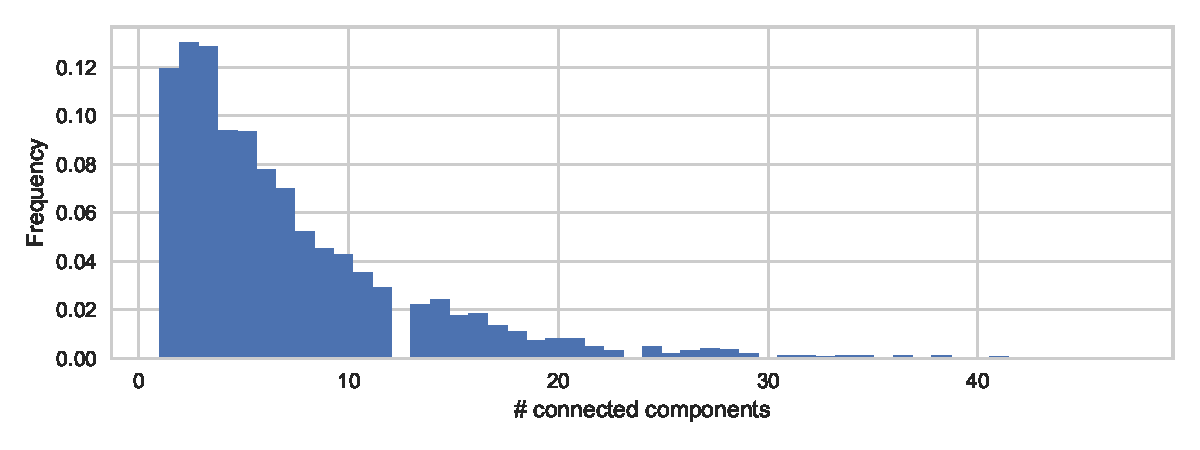
\includegraphics[width=0.8\linewidth]{assets/figures/hist-connected-components-ling-spam-CMap.pdf}
\caption[Statistics: Histogram of connected components per concept map]{Histogram of connected components per concept map. Dataset: \textit{ling-spam}.}\label{fig:histogram_connected_components}
\end{figure}

\begin{figure}[htb!]
	\centering
	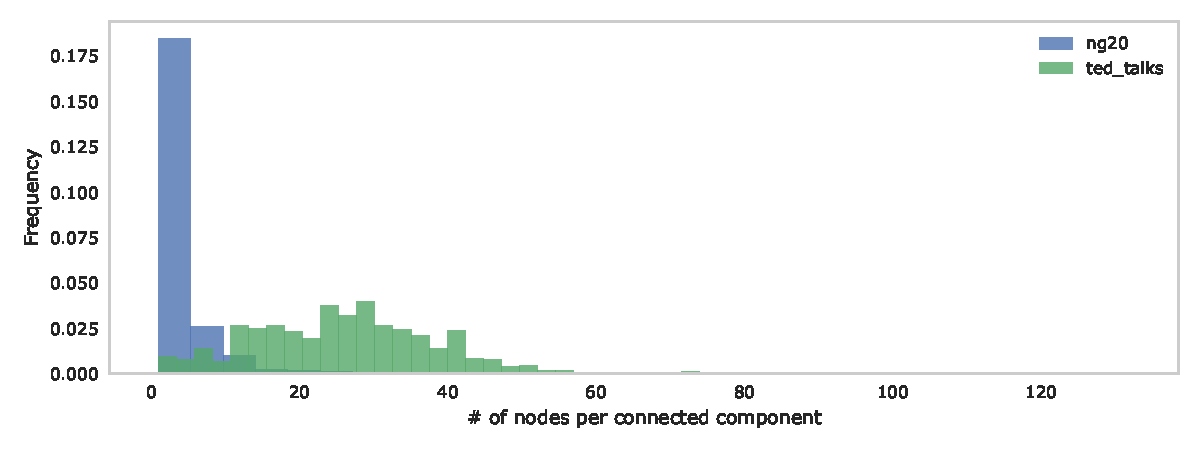
\includegraphics[width=0.9\linewidth]{assets/figures/connected_component_size_comparison.pdf}
	\caption[Statistics: Histogram of size of connectec components]{Histogram of the size of connected components, ie. the number of nodes per connected component, of concept maps for two datasets. The distribution of the size of connected components varies greatly between different datasets. In this instance, the \textit{ng20} dataset has mostly small connected components while the \textit{ted\_talks} dataset has bigger connected components. This is most likely due to the fact that the \textit{ted\_talks} dataset consists of longer, more coherent texts while the \textit{ng20} texts are shorter as well as more informal, leading to fewer recurring concepts.}
	\label{fig:histogram_connected_component_size}
\end{figure}

\begin{figure}[htb!]
\centering
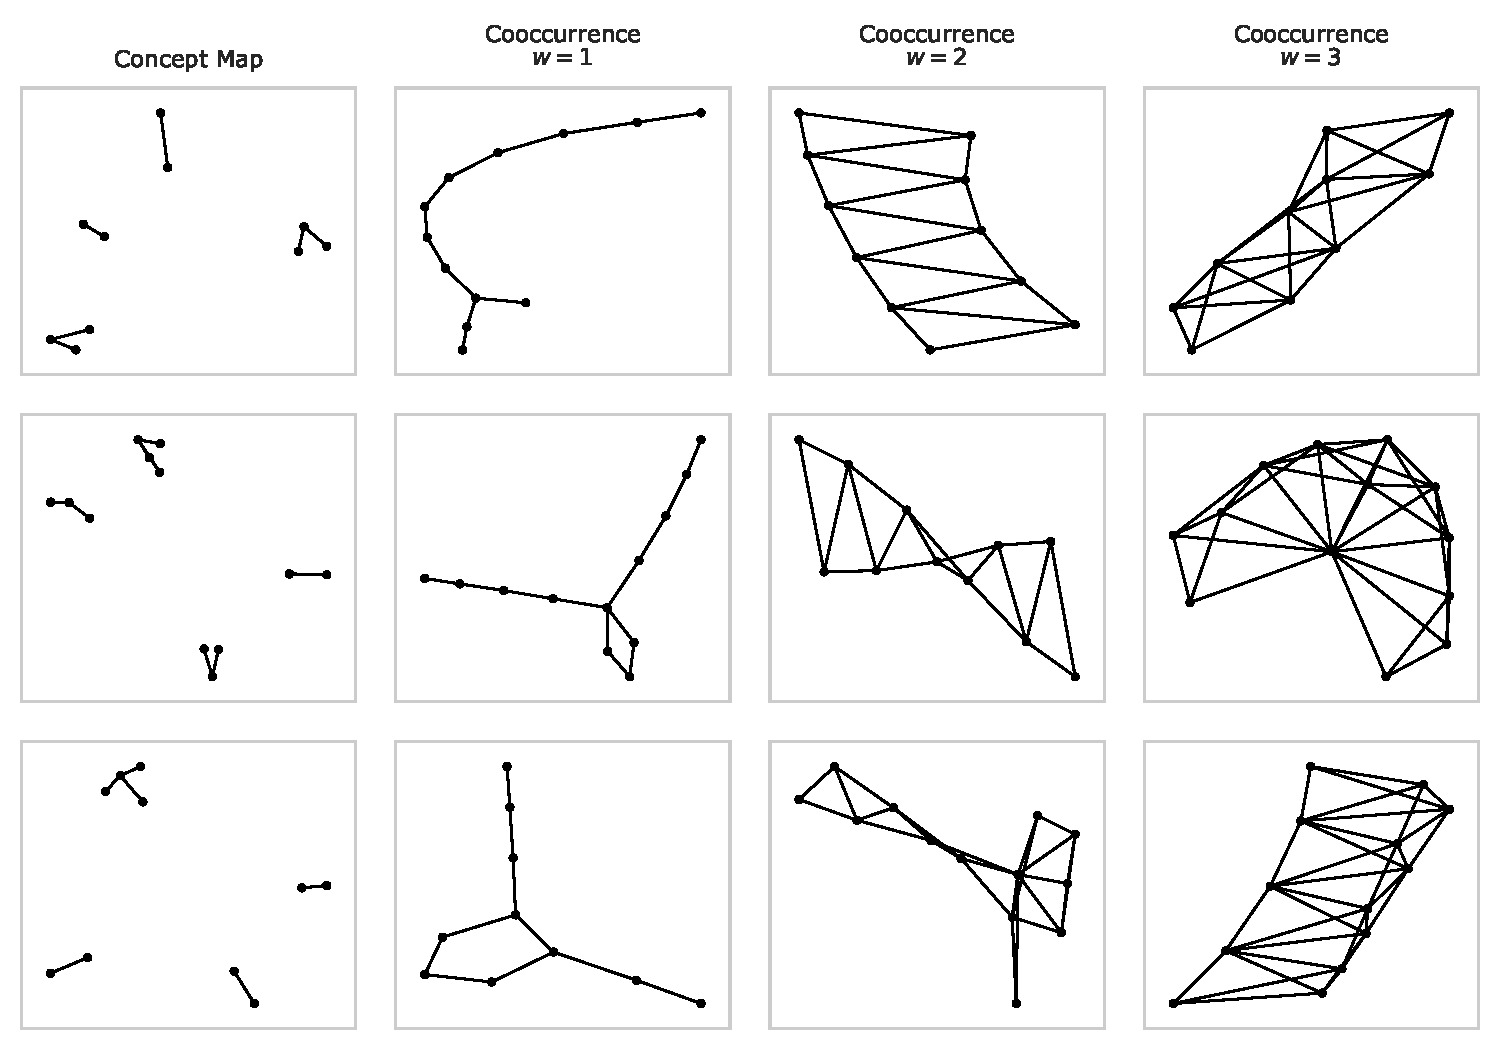
\includegraphics[width=0.8\linewidth]{assets/figures/examples_graphs.pdf}
\caption[Examples: Graph types]{Graph examples per type. Three random examples are shown per type. $w$ stands for the window size of the co-occurrence graph. The concept map examples all have more than one connected component, while all co-occurrence graphs have only one. The shown graphs were randomly chosen from all graphs with $5 \leq |V| \leq 10$.Dataset: \textit{ng20}}\label{fig:graph_examples}
\end{figure}

\begin{figure}[htb!]
\centering
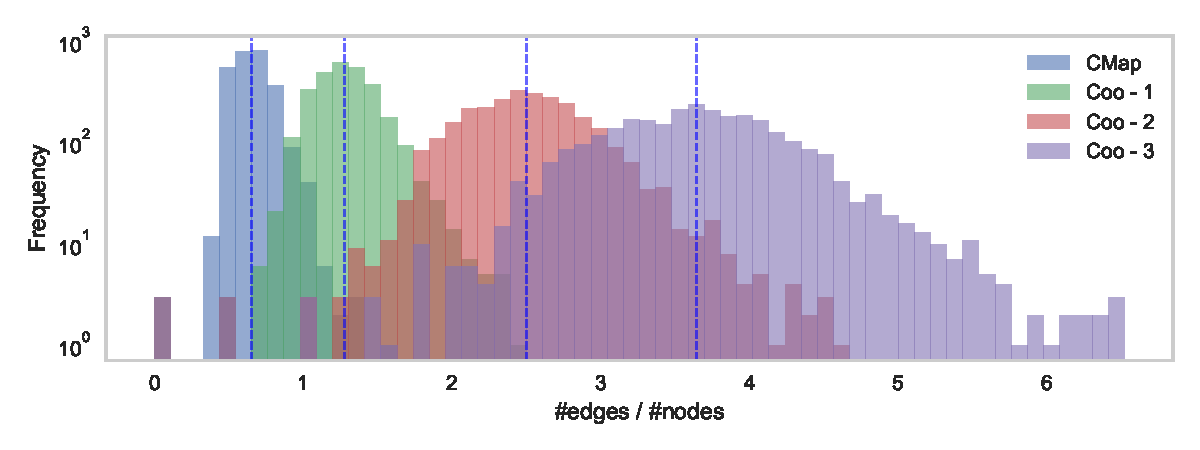
\includegraphics[width=0.7\linewidth]{assets/figures/hist-edgesnodes.pdf}
\caption[Statistics: Histogram of the number of edges divided by the number of nodes]{Histogram of the number of edges divided by the number of nodes. Per graph type. The lines correspond to the median value.}
\label{fig:histogram-edges-div-nodes-per-type}
\end{figure}

The co-occurrence graphs also have a simple structure.
Co-occurrence graphs are always connected, ie. the number of connected components is 1, or 0 in the case of an empty graph.
When the window size is 1, the graph is similar to a path, meaning that most of the nodes have a degree $< 2$. With increasing window size, the graph also gets more connected.

\answersummary{
Concept maps have a relatively homogeneous structure.
The bulk of its nodes have only a small number of neighbors.
The degrees of nodes are quite low, also hinting that there are few recurring concepts.
}

\subquestionref{question:importance_structure}
After investigating the structure of concept maps, we now aim to quantify the importance of the structure compared to the content.
The content, that is the node and edge labels, of concept maps are also captured in co-occurrence graphs and with conventional text-based approaches. So, the next interesting question about concept maps is, how much or whether the structure adds to the classification performance.
For this, we compare the results of using graph kernels which use \textbf{(a)} only the content, \textbf{(b)} only the structure and \textbf{(c)} both content and structure.

For \textbf{(a)} (content only), we use a kernel that discards all edges and uses only the labels of nodes and edges. Next, we create a bag-of-words vector representation out of the labels and edges.
In this step, we also evaluated using not only single words and counting them, but also using word n-grams of size 2, or bi-grams.
For this, we create pairs of words by joining node labels together that have an edge between them.
The resulting vector representations of the graph then get fed into a conventional classifier, in our case a SVM.

For \textbf{(b)} (structure only), we use a modified version of the Weisfeiler-Lehman graph kernel. Before applying the actual WL kernel, we discard all node labels and give every node in all graphs the same label, effectively ridding the graphs of content. Next, we apply the WL graph kernel. This variant of WL only takes the structure of the graph into account.
After executing WL on the graphs, we obtain the feature maps which get subsequently get fed into a SVM also.

For \textbf{(c)} (structure and content combined), we use the Weisfeiler-Lehman that takes both structure and content into account.

In Table \ref{table:table_results_structure_vs_content} we report the results obtained from these experiments.

\begin{table}[htb!]
\centering
\begin{tabular}{llrrr|r}
\toprule
          & & \multicolumn{4}{c}{f1 macro} \\
Dataset & Type & \textbf{(a)} content only & \textbf{(b)} structure only & \textbf{(c)} combined & Dummy\\
\midrule
ling-spam & Concept Map & 0.934 & 0.544 & 0.816 & \multirow{2}{*}{0.421} \\
& Cooccurrence & 0.997 & 0.620 & 0.987 & \\
\midrule
ng20 & Concept Map & 0.622 & 0.057 & 0.419 & \multirow{2}{*}{0.051} \\
& Cooccurrence & 0.627 & 0.068 & 0.593 & \\
\midrule
nyt\_200 & Concept Map & 0.899 & 0.324 & 0.744 & \multirow{2}{*}{0.170} \\
& Cooccurrence & 0.891 & 0.422 & 0.881 & \\
\midrule
r8 & Concept Map & 0.892 & 0.184 & 0.677 & \multirow{2}{*}{0.087} \\
& Cooccurrence & 0.890 & 0.300 & 0.890 & \\
\midrule
review\_polarity & Concept Map & 0.737 & 0.575 & 0.609 & \multirow{2}{*}{0.502} \\
& Cooccurrence & 0.762 & 0.526 & 0.785 & \\
\midrule
rotten\_imdb & Concept Map & 0.828 & 0.579 & 0.635 & \multirow{2}{*}{0.504} \\
& Cooccurrence & 0.831 & 0.561 & 0.825 & \\
\midrule
ted\_talks & Concept Map & 0.359 & 0.279 & 0.244 & \multirow{2}{*}{0.236} \\
& Cooccurrence & 0.461 & 0.141 & 0.443 & \\
\bottomrule
\end{tabular}
\caption[Results: Linearized vs. WL]{Results for linearized graphs. \textit{Combined} are features generated using plain WL, using both structure and content. With \textit{Structure-only}, all node labels are omitted, then also plain WL. \textit{Content-only} linearizes the graph into text, then does conventional BoW feature extraction.}\label{table:table_results_structure_vs_content}
\end{table}

Here, we see that the content-only approach works the best for both concept maps and cooccurrence graphs.
The structure-only approach performs far worse, nearly as worse as the dummy classifier which only predicts the most-common label.
The combined approach, ie. plain WL, performs better than the structure-only but worse than the content-only approach.

While it is no surprise that removing the labels from the graphs results in a far lower classification score, the extent in which co-occurrence graphs still perform better than concept maps has to be noted.
This could indicate that the structure of co-occurrence graphs, while relatively simple, might also be useful for classification.

\answersummary{
The content-only graph kernel, which un-rolls the graph into text and then uses a conventional uni-gram \textit{BoW} vectorizer approach, performs the best for both concept maps and co-occurrence graphs.
Removing the content, ie. the labels, from the graphs and then running WL results in classification scores comparable to the most-frequent dummy classifier.
When combining both, content and structure, ie. plain WL, the score is lower than content-only.
This all indicates that the content of the graphs, for graph-only classification, has a greater importance than the structure since the structure gets completely discarded by the content-only approach and still performs the best.
}

\subquestionref{question:multi_labels}
In Figure \ref{fig:statistics_percentage_multi_word_labels} we see, that most concept map node labels consist of more than one word.

\begin{figure}[htb!]
	\centering
	\includegraphics[width=0.7\linewidth]{assets/figures/tmp/statistics_percentage_multi_word_labels.pdf}
	\caption[Statistics: Percentage multi-word node labels]{Percentage of multi-word to single-word node labels per dataset.}\label{fig:statistics_percentage_multi_word_labels}
\end{figure}

However, with the normal approach, like counting the node labels, these multi-word labels are treated as single labels, effectively discarding important information.
In the experiments of the last question, Question \ref{question:importance_structure}, we actually implicitly used the multi-word labels since we un-rolled the graph into text again and then used conventional text vectorizer, ie. BoW.
In these experiments, we saw an improvement over the graph based approach, possibly due to the multi-word labels being split.
So, for our next graph-based approach, we also split nodes with multi-word labels into multiple single-word nodes.
This is done by splitting the node labels into individual words, than creating nodes with these single words and adding all the (directed) edges of the original node.
When a resulting single-word label is a stopword, the corresponding node is removed from the graph.
See Figure \ref{fig:example_split_labels} for an example.

Additionally, we also evaluate the stemming or lemmatizing [p.~4]\cite{Manning2000} the split single-words.

\begin{figure}[htb!]
	\centering
	\begin{subfigure}[t]{.4\linewidth}	{\includegraphics[width=\linewidth]{assets/figures/tmp/graph_example_split_labels_before.pdf}}
		\caption{Before}
	\end{subfigure}
\hspace{2cm}
	\begin{subfigure}[t]{.4\linewidth}	{\includegraphics[width=\linewidth]{assets/figures/tmp/graph_example_split_labels_after.pdf}}
		\caption{After}
	\end{subfigure}
	\caption[Example: Multi-word node labels Splitting]{Example for multi-word label splits. Here, both the ``concept maps" and ``multi-word concepts" node labels are  split.}\label{fig:example_split_labels}
\end{figure}

In Figure \ref{table:results_multi_label_split} we report the results when doing graph classification with and without multi-word label splitting.
For this experiment, we use the Weisfeiler-Lehman graph kernel to extract the feature maps.
As we can see, the splitting actually improves the performance quite a lot, consistently outperforming the non-split version on all datasets.
On some datasets, the additional stemming of single-word labels after splitting also further improves the score.

\begin{table}[htb!]
	\centering
\begin{tabular}{lrrrr}
\toprule
	{} & \multicolumn{3}{c}{F1 macro}  &   \\
	 &  Un-Split  &  Un-Stemmed &  Stemmed &   $p$-Value  \\
	\midrule
	ling-spam       & 0.8160 & 0.8835 & \textbf{0.9131} & 0.0008 \\
	ng20            & 0.4188 & 0.5680 & \textbf{0.5741} & 0.0001 \\
	nyt\_200         & 0.7436 & \textbf{0.8464} & 0.8294 & 0.0001 \\
	r8              & 0.6772 & \textbf{0.8599} & 0.8441 & 0.0001 \\
	review\_polarity & 0.6094 & \textbf{0.7150} & 0.6699 & 0.0036 \\
	rotten\_imdb     & 0.6346 & \textbf{0.7805} & 0.7775 & 0.0001 \\
	ted\_talks       & 0.2436 & 0.3934 & \textbf{0.4126} & 0.0035 \\
	\bottomrule
\end{tabular}
\caption[Results: Multi-label split]{Results for multi-label node label split. The $p$-value is calculated with the best split-word approach, ie. stemmed and un-stemmed, versus the plain version.}\label{table:results_multi_label_split}
\end{table}

The classification scores for this multi-word splitting nearly performs as well as the linearized, BoW approach from the previous Question \ref{question:importance_structure}, ranging from 1\% to 3\% difference in F1 macro.
However, it has to be noted that splitting the multi-word node labels, and subsequently extracting features with WL, produces higher dimensional feature vectors than the un-split approach.


\answersummary{
Splitting the multi-word labels shows the greatest performance improvement for WL, ranging from a raise of 10\% to 24\% better F1 macro score over the un-split approach.
Splitting the node labels and then using WL performs nearly as good as the best graph kernel we saw, the linearized content-only approach from Question \ref{question:importance_structure}.
}

\subquestionref{question:edge_labels}
To evaluate how important the edge labels are, we first look at the occurrences of edge labels, ie. how often a unique edge label occurs in the concept maps of a whole dataset.
In Table \ref{table:edge_label_occurrences} we see that, on average, 76\% of all unique edge labels occur only once per dataset. For comparison, the percentage of unique words which only occur once in a text, on average, is often well below 50\% for our datasets.

\begin{table}[htb!]
	\centering
	\begin{tabular}{lrr}
\toprule
		dataset &  $ \%_{unique} $ & $ \%_{all}$  \\
		\midrule
		ling-spam       & 69 & 27 \\
		ng20            & 73 & 30 \\
		nyt\_middle      & 73 & 32 \\
		nyt\_small       & 78 & 43 \\
		review\_polarity & 80 & 39 \\
		rotten\_imdb     & 80 & 47 \\
		tagmynews       & 75 & 39 \\
		ted\_talks       & 80 & 39 \\
		\midrule
		\O           & 76 & 37 \\
		\bottomrule
	\end{tabular}
	\caption[Statistics: Percentage of concept map labels occurring once]{Percentage of concept map edge labels occurring only once in the whole dataset.
		$ \%_{unique} $ corresponds to the percentage of edge labels which only occur once to the number of unique labels in the whole dataset, eg. $ \%_{unique} = 50\% $ would mean that 50\% of all unique edge labels occur only once.
		$ \%_{all}$ stands for the percentage of edge labels which occur only once to all labels (with duplicates), eg. $ \%_{all} = 50\%$ would mean that 50\% of all edge labels occur only once in the dataset.}\label{table:edge_label_occurrences}
\end{table}

When examining the most occurring edge labels per dataset, most of these most-frequent edge labels consist of stopwords or non-descriptive words like ``is", ``has", ``are".
These most-frequent edge labels, together with the edge labels which occur only once, form the bulk of all edge labels.

As a test for the importance of edge labels, we evaluate \textbf{(a)} a graph kernel which uses the edge labels against \textbf{(b)} a graph kernel which does not use edge labels.
For both, \textbf{(a)} and \textbf{(b)}, we use a graph kernel which first converts the graphs into a text and then vectorizes the text with BoW, introduced in Question \ref{question:importance_structure}.
For \textbf{(a)} we use the edge labels for the text, for \textbf{(b)} we omit them.

\begin{table}[htb!]
	\centering
\begin{tabular}{lrrr}
\toprule
	{} & \multicolumn{2}{c}{Edge Labels}  & p-value \\
	{}	& without & with & {} \\
	\midrule
		ling-spam       & \textbf{0.898} & 0.896 & 0.830 \\
		ng20            & 0.620 & \textbf{0.624} & 0.502 \\
		nyt\_200         & \textbf{*0.900} & 0.875 & 0.031 \\
		r8              & 0.882 & \textbf{0.883} & 0.959 \\
		review\_polarity & 0.700 & \textbf{0.727} & 0.271 \\
		rotten\_imdb     & 0.817 & \textbf{0.823} & 0.533 \\
		ted\_talks       & \textbf{0.410} & 0.363 & 0.164 \\
	\bottomrule
\end{tabular}
\caption[Results: Graph Kernel with and without edge labels]{Classification results concept maps using a graph kernel with and without edge labels.  The star * signifies results where the model is significantly better under the permutation test ($p = 0.05$)}\label{table:edge_label_classification}
\end{table}

As we can see in Table \ref{table:edge_label_classification}, omitting or using the edge labels results in non-significant differences in classification performance.
For some datasets, omitting the edge label actually even improves the classification score.
These facts all indicate that edge labels, while crucial and useful for text-summarization and the subsequent use by a human, seem to have limited use in graph classification.

\answersummary{
		The bulk of all edge labels either occurs only once per dataset or consists of stopwords.
		In our experiments, omitting or using the edge labels actually leads to comparable performances.
}

\subquestionref{question:infrequent_nodelabels}
In Figure \ref{fig:percentage_distribution_concept_occurrences} we can see that, depending on the dataset, between 75\% to 90\% of all node labels occur only once per dataset.
This is also common in texts where most words also only occur once per dataset.
 
\begin{figure}[htb!]
	\centering{\includegraphics[width=\linewidth]{assets/figures/tmp/percentage_distribution_concept_occurrences.pdf}}
	\caption[Statistics: Distribution concept occurrence]{Concept map node label occurrences per dataset. $|n_v| = i$ stands for the percentage of labels with $i$ occurrences in the dataset, eg. when $|n_v| = 1$ has 50\%, it would mean that 50\% of all unique concepts only occur once per dataset.}\label{fig:percentage_distribution_concept_occurrences}
\end{figure}

In text-based approaches, infrequent words are either ignored or filtered out to reduce the vocabulary and subsequently the dimension of the feature vector
Yet, for our approach, infrequent node labels might pose a far greater problem.
As noted before, in our work, we capitalize on the Weisfeiler-Lehman graph kernel to extract useful features for subsequent classification.
In the context of WL, infrequent node labels might become a problem since a match becomes less likely with fewer occurring words, or a match even becomes impossible as in the case of node labels which occur only once.
When simply creating a feature vector by counting the node labels in each graph, infrequent node labels would not pose a problem.
WL on the other hand relies on exact matches of neighborhoods.
Thus, a node label which only occurs once would ``taint" its neighborhood, effectively making matches in its neighborhoods impossible.

In Table \ref{table:results_infrequent_nodes} we see the results of removing infrequent labels.

\begin{table}[htb!]
	\centering
	\begin{tabular}{lrrr}
\toprule
		&  \multicolumn{2}{c}{F1 macro} &  \\
		 &  Plain &  Removed &  $p$-value \\
		\midrule
			ling-spam       & 0.8105 & 0.8064 & 0.6835 \\
			ng20            & *0.4157 & 0.3536 & 0.0002 \\
			nyt\_200         & 0.7601 & 0.7640 & 0.8466 \\
			r8              & 0.6774 & 0.6421 & 0.0720 \\
			review\_polarity & 0.6025 & 0.6066 & 0.8868 \\
			rotten\_imdb     & *0.6373 & 0.5494 & 0.0002 \\
			ted\_talks       & 0.2449 & *0.3687 & 0.0062 \\
		\bottomrule
	\end{tabular}
	\caption[Results: Remove infrequent node labels]{Classification results with infrequent nodes removed.}\label{table:results_infrequent_nodes}
\end{table}

As we can see, removing the node labels results in a lower score for most datasets, except for the \textit{ted\_talks} corpus.

\answersummary{
	TODO	
}

\subquestionref{question:relabeling_infrequent}
In the previous question, we looked at infrequent node labels and removed them.
For this question, we actually merge infrequent nodes label with other, more frequent nodes labels.
To do this, we have to find a measure of similarity between two node labels to determine whether they should be merged or not.
There are a great number of approaches to define similarity between two word labels, eg. for example the edit distance between word sequences.
For our purpose, we use word embeddings \cite{Mikolov2013,Pennington,Goldberg2014} to obtain a measure of similarity between multi-word labels.
We leverage the pre-trained word embeddings introduced and provided in \cite{Pennington}.
Each word $w$ in the vocabulary of the pre-trained word embedding has a relatively low-dimensional vector $v_w$ assigned, the embedding.
Roughly speaking, the intuition of word embeddings is that when an word $w$ is semantically similar to another word $w'$, the distance $|| v_w - v_w' ||$ between their embeddings is low, while dissimilar words have higher distances.
Pre-trained word embeddings, as a downside, have a fixed vocabulary.
So, we actually have two problems when using word embeddings for our multi-word node labels, namely (1) we have multi-word labels, while our pre-trained word embeddings only contain single single-word embeddings, (2) some node labels will not be in the vocabulary of the pre-trained vocabulary.
Preliminary tests show us that both problems, (1) and (2), are very common in our datasets and therefor must be addressed.

\paragraph{Multi-Word and Missing Node Label Lookup}
Our idea to solve these issues was to first create a Word2Vec \cite{Mikolov2013} word embedding \textit{(TrainedEmbedding)} from the texts in the datasets.
In the next step, we resolve (1) multi-word labels and (2) labels which are not in the vocabulary of the pre-trained word embedding \textit{(Pretrained Embedding)}.
For each node label $n$, (a) we split $n$ into single words if it is a multi-word label and then (b) obtain the embeddings for the single words from the \textit{(TrainedEmbedding)}, then (c) create the average of the found embeddings.
If the node label contains only one word, we need not average the found embeddings.
So, in this stage we have obtained a (multi-) word embedding $v_n$ for the node label $n$ from the  \textit{(TrainedEmbedding)}.
Next, we search for similar words $ws$ to $v_n$ with the constraint that each word in $ws$ also has to be in the \textit{(Pretrained Embedding)}.
We obtain the similar words by using the multi-word embedding $v_n$ to search for similar word embeddings in the \textit{(TrainedEmbedding)}.
The similar words $ws$ also contain the similarity between the nodes, ie. their distance.
We only keep the top $n$ similar words in $ws$. In our case, $n = 10$.

So, at this stage, for each (multi-word) node label $n$ in the concept maps, we have similar words $ws_n$ which are both in the \textit{(Pretrained Embedding)} and the \textit{(TrainedEmbedding)}.
Now, we solved both problems, (1) the multi-word labels and (2) words which are not in the vocabulary of the \textit{(Pretrained Embedding)}.

\paragraph{Node Label Clustering}
In the next step, we have to find node label sets which should be merged.
For this, we greedily merge labels into clusters with unique identifiers, eg. consecutive numbers, where each label $n$ in a cluster have a similarity, or distance, greater than a given threshold, $t$, to \textit{any} node label in the cluster.
After this step, each node label in the concept maps has a assigned cluster with one or more node labels in it.
The intuition of these clusters is that a cluster only contains similar labels.
This also means that we could merge the labels in some cluster.

\paragraph{Infrequent Node Label Merging}
So now, we actually can replace infrequent node labels with the cluster identifier.
We also replace each node label in that cluster with 
Assuming that both the \textit{(TrainedEmbedding)} and the \textit{(Pretrained Embedding)} actually capture semantical similarities, this new label will be semantically similar to the original, but infrequent node label.

\paragraph{Discussion}
There are several assumptions made here for this approach to be useful, namely that a semantically meaningful word embedding for infrequent node labels can be obtained.
When a node label only occurs once in the whole dataset, creating a meaningful word embedding for this single occurrence can be quite difficult since word embeddings actually work by defining a word by its context.
Yet, in this instance, we have only one context since the node label occurs only once.
That said, this caveat only applies partially since most of the node labels we merge actually are multi-word labels and the individual words in them occur, most likely, more than once.
Another important caveat to keep in mind is that we used the complete text corpus to train our \textit{(TrainedEmbedding)}.
This means that we did no trainings- and validation split nor cross-validation at all.
This was done to reduce the already quite high compute time of training the embeddings and merging them.
The results are most likely tainted by the omission of the clear separation between train- and test data.

\paragraph{Results}
After relabeling the infrequent labels as explained above, we then use our default approach, applying WL to the relabeled concept maps to obtain feature maps, then classifying them.
As a baseline, we also apply the same approach to un-relabeled concept maps.
In Table \ref{table:results_infrequent_relabeled} we report our results.
For the experiments, we tested different thresholds $t \in \{0.5, 0.7, 0.9\}$ and $n=10$, that is we only considered the top-10 words when creating the new embeddings, see above.

\begin{table}[htb!]
	\centering
	\begin{tabular}{lrrrr}
\toprule
		{} & \multicolumn{3}{c}{F1 Macro} &  \\
		Threshold $t$ &         0.5 &   0.9 & Plain & p-value \\
		\midrule
		ling-spam       & \textbf{0.831} & 0.817 & 0.816 & 0.515 \\
		ng20            & 0.377 & 0.383 & \textbf{*0.419} & 0.000 \\
		nyt\_200         & 0.739 & 0.727 & \textbf{0.744} & 0.885 \\
		r8              & \textbf{0.705} & 0.693 & 0.677 & 0.268 \\
		review\_polarity & \textbf{0.616} & 0.606 & 0.609 & 0.780 \\
		rotten\_imdb     & 0.577 & 0.605 & \textbf{0.635} & 0.194 \\
		ted\_talks       & 0.281 & \textbf{0.317} & 0.244 & 0.188 \\
		\bottomrule
	\end{tabular}
	\caption[Results: Merge infrequent nodes]{Classification results for relabeled concept maps. The $p$-value is obtained by a significance test between the plain and the best relabeled version, eg. 0.5 or 0.9. Plain corresponds to the un-relabeled approach.	}
	\label{table:results_infrequent_relabeled}
\end{table}

As we can see, on some datasets, relabeling the nodes can improve the classification score, while others do not profit from this additional pre-processing step.

\answersummary{
	After devising and applying an approach to merge (multi-word) node labels of concept maps, we classify them.
	In most datasets, this results in a significant improvement in classification performance.
	Nevertheless, there are also big caveats to this approach, for instance the additional overhead of computing word embeddings for the whole dataset.
}

\subquestionref{question:directed_vs_undirected}
The concept maps we extracted have directed edges.
In this question, we evaluate the usefulness of these two cases.
We compare the classification performance of using the directed versus un-directed case with the Weisfeiler-Lehman graph kernel.

When using WL with undirected edges, the neighbors $n_v$ of a node $v$ are all nodes $v'$ that are connected by an edge to $v$, or $n_v = \{v' | (v, v') \in E \lor (v', v ) \in E \}$.
With directed edges, on the other hand, the neighbors $n_v$ of a node $v$ are only nodes $v'$ where there exists a directed edge from $v$ to $v'$, or $n_v = \{v' | (v, v') \in E \}$.
So, the size of neighborhoods per node are expected to decrease, since there is an additional constraint to what constitutes a neighbor.

In Table \ref{table:results_directed_vs_undirected} we see the results of using WL with directed and un-directed edges.
On all datasets, the directed edges outperform the un-directed ones.

\begin{table}[htb!]
	\centering
\begin{tabular}{lrr}
\toprule
	&  \multicolumn{2}{c}{F1 macro} \\
	 &  un-directed & directed \\
	\midrule
ling-spam       & 0.748 & 0.816 \\
ng20            & 0.416 & 0.419 \\
nyt\_200         & 0.743 & 0.744 \\
r8              & 0.576 & 0.677 \\
review\_polarity & 0.581 & 0.609 \\
rotten\_imdb     & 0.633 & 0.635 \\
ted\_talks       & 0.219 & 0.244 \\
	\bottomrule
\end{tabular}
\caption[Results: WL with directed and un-directed edges]{Classification results when using directed versus un-directed edges with WL.}\label{table:results_directed_vs_undirected}
\end{table}

This is most likely due to the aforementioned property that the neighborhoods are smaller with directed edges, making exact matches of neighborhoods more probable.
\todo{
Note that using directed edges in WL could be compared with using n-grams since they also are directed.
Instead of word n-grams these are concept n-grams, consisting of three components, the two sink and target vertex labels plus the edge label between them.
For bigger WL iterations, these concept 3-grams then capture longer $n$-grams and so on.
}
When the order of words/nodes is fixed in one direction, vertices with no outgoing edges do not have a neighborhood. Thus they are, for all WL iterations, considered to be the same label, ie. they get no new color assigned.

As a result of these better classification results with directed edges, we will use the directed version of WL.
Later on, we will also evaluate whether or how using (un-) directed edges affects the score when combining graph and text features.


\answersummary{
 	Using directed instead of un-directed edges results in significantly better performance with the WL graph kernel.
 	A possible explanation for this better performance is that neighborhood matches with directed edges are far easier since the neighborhood of a vertex is only defined through its outgoing edges, and not the in-going as well.
 	The smaller neighborhood in turn makes exact matches of neighborhoods in different graphs more probable.
}

\subquestionref{question:concept_map_size}
In most datasets, longer texts often result in higher classification performance.
So, an interesting question is whether the size of a concept map also correlates with its classification performance, ie. whether ``bigger" graphs in terms of the number of nodes and edges are easier to classify.
To test this, we classify the graphs with our standard approach, using the Weisfeiler-Lehman graph kernel, then a SVM to classify the feature maps.
For text, we extract the features with Tfidf-BoW, then also classify the features with a SVM.

% IGNORED
\iffalse
In the next step, we look at the results for different graph sizes, binning them with quantiles, in our case 10 quantiles, or deciles.

\begin{figure}[htb!]
	\begin{subfigure}[t]{.5\linewidth}	{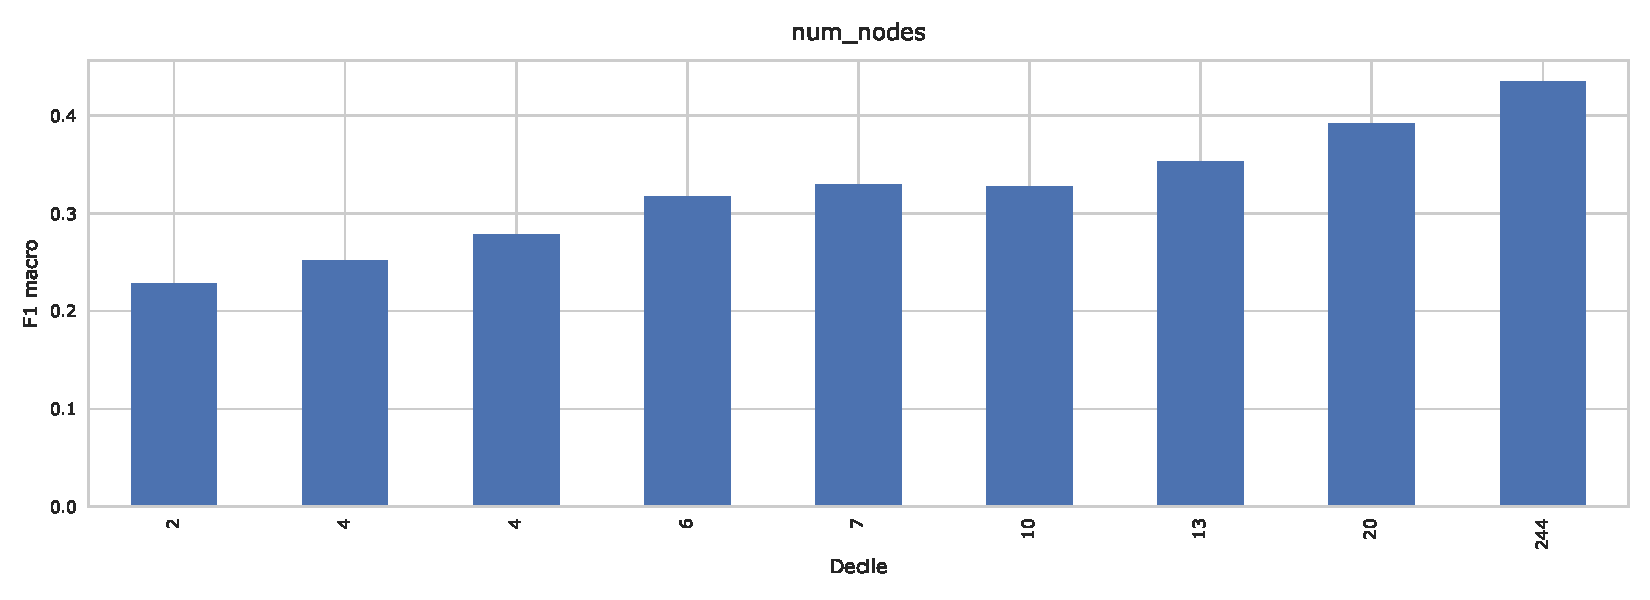
\includegraphics[width=\linewidth]{assets/figures/graph_binning_num_nodes.pdf}\label{fig:todo_1}}
	\caption{Graphs}
	\end{subfigure}
	\hfill
		\begin{subfigure}[t]{.5\linewidth}
	{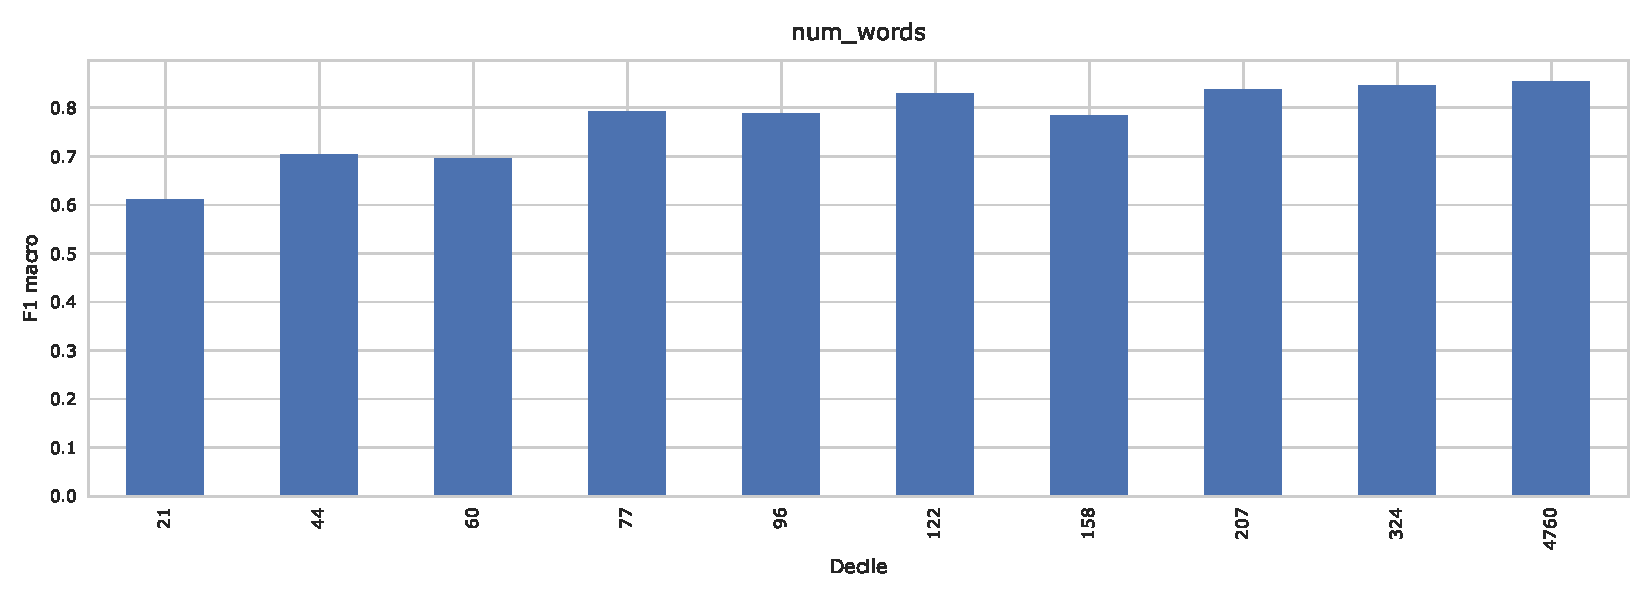
\includegraphics[width=\linewidth]{assets/figures/text_binning_num_words.pdf}\label{fig:todo_2}}
	\caption{Text}
	\end{subfigure}
	\caption[Statistics: Histogram of classification performance per graph/text size]{Classification performance per graph/text size. The x-axis corresponds to the size of the graph/text, the y-axis for the classification performance for graphs/text of that size. Dataset: \textit{ng20}}\label{fig:graph_size_performance}
\end{figure}


For the \textit{ng20} dataset, the results indicate that classification performance indeed correlates with the number of vertices.
In other datasets, this correlation is not as distinguished.
\fi

In Table \ref{table:correlations_size} we report the Spearman rank correlations \cite{Hauke2011} between the accuracy, ie. whether the label for the document/graph was predicted right, and the size of the document/graph.
Here, we also see a (weak) correlation for the graph sizes in some datasets.
In the \textit{ling-spam} and \textit{ng20} dataset, the accuracy correlates far more with the document/graph size than in other datasets.
It has to be noted that there is no partial similarity in accuracy, only 1 if the label was predicted right and 0 otherwise.
This might also explain that the relatively low correlation between the graph/document size and the accuracy, even in \textit{ng20}.

These results also highlights another finding: one observation for some dataset might not be consistent with observations from another dataset, eg. for our results the correlations are sometimes weak, sometimes practically not present at all.

We also tested other metrics to find correlations, for instance the number of edges or the number of connected components, yet we could not see relevant correlations.

\begin{table}[htb!]
	\centering
	\begin{tabular}{lrr}
\toprule
		&  \multicolumn{2}{c}{Spearman correlation} \\
		&  Graph &  Text \\
		\midrule
		ling-spam       &  0.2135 &  0.1490 \\
		ng20            &  0.2699 &  0.2415 \\
		nyt\_200         & -0.1986 &  0.0077 \\
		r8              & -0.0212 & -0.0499 \\
		review\_polarity & -0.0311 & -0.0286 \\
		rotten\_imdb     &  0.1680 &  0.0313 \\
		ted\_talks       & -0.0232 & -0.0991 \\
		\bottomrule
	\end{tabular}
	\caption[Table: Graph/text size correlations]{Spearman rank correlations between the accuracy and graph/text size. Here, the graph size is the number of nodes in the graph, text size the number of words. The higher the absolute value of the Spearman correlation is to 1, the higher the correlation.
	A positive correlation value between A and B means that if A increases, B also increases and vice versa.
	A negative correlation means that when A increases, B decreases and vice versa.}%
	\label{table:correlations_size}
\end{table}

\answersummary{
	In some datasets, we see a correlation between the size of graph/documents and the prediction accuracy.
	For other datasets, this correlation can not be measured distinctly.
	The results vary widely across datasets. 
}

\subquestionref{question:comparison_coo}
As a baseline, we also look at another graph representation for text, namely co-occurrence graphs.
The comparison between concept maps and co-occurrence graphs is somewhat unfair since co-occurrence graphs retain much more of the content of its underlying text.
While both concept maps and co-occurrence graph are graph representations, they have several differences. While concept maps have directed edges with labels, co-occurrence edges are, in the our version, undirected and have no edge labels.
The node labels for concept maps also contain multiple words while co-occurrence graphs have single-word labels per definition.

We use the comparison of co-occurrence graphs to concept maps to establish a baseline for graph representations.
Since our main hypothesis assumes that concept maps contain useful structural information, the co-occurrence graph is a good candidate for comparison, since its structure is quite simple.
For window size $w=1$, the co-occurrence graphs have a mainly linear structure. With higher window sizes, the co-occurrence graphs get more connected until they eventually become fully connected.

In Table \ref{table:comparison_results_cooccurrence} we report our results.


\begin{table}[htb!]
	\centering
	\begin{tabular}{lcc|c}
	\toprule
		{} &  \multicolumn{2}{c}{F1 macro} \\
		& Concept &  Co-Occurrence & Difference \\
		\midrule
			ling-spam       & 0.816 & 0.987 & 0.171 \\
			ng20            & 0.419 & 0.593 & 0.174 \\
			nyt\_200         & 0.744 & 0.881 & 0.138 \\
			r8              & 0.677 & 0.890 & 0.213 \\
			review\_polarity & 0.609 & 0.785 & 0.175 \\
			rotten\_imdb     & 0.635 & 0.825 & 0.191 \\
			ted\_talks       & 0.244 & 0.443 & 0.199 \\
		\bottomrule
	\end{tabular}
	\caption[Results: Co-Occurrence vs. Concept Maps]{Classification scores for co-occurrence graphs and concept maps.}\label{table:comparison_results_cooccurrence}
\end{table}

As we can see, graph classification using co-occurrence graphs performs significantly better than the concept maps.
Co-occurrence graphs also perform nearly as good as the conventional, text-based approach.
That said, co-occurrence graphs contain far more information than concepts, as we have seen in Table \ref{table:graph_statistics}.
Concept maps on the other hand summarize the text by filtering out only important concepts.
Conversely, co-occurrence graphs actually contain all words of its underlying text.
For this comparison, we used co-occurrence graphs where we only keep the nouns of the text to mimic the summarization of concept maps.
Apart from that, since co-occurrence graphs contain more information, creating the feature maps with WL also incurs more compute time.

\answersummary{
	Using WL, co-occurrence graphs perform far better than concept maps in graph-only classification.
	One explanation is that co-occurrence graphs actually retain more information about the text, ie. all words and their co-occurrence, while concept maps have a far higher compression factor, even though the co-occurrence graphs were created from nouns-only.
	However, this increased number of nodes/edges in co-occurrence graphs also increase the runtime and memory footprint while extracting the WL features.
}

\subquestionref{question:comparison_text}
As one can see in Figure \ref{fig:results_cmap_vs_text}, the text-only approach outperforms graph-only approaches by a high margin.
This is most likely due to the high compression factor of both concept maps and co-occurrence graphs.

\begin{table}[htb!]
	\centering
	\begin{tabular}{lrrrr}
		\toprule
		 & \multicolumn{4}{c}{F1 macro} \\
		type &  Concept &  Co-Occurrence & Text (Count) & Text (Tfidf) \\
		\midrule
		ling-spam       & 0.816 & 0.987 & 0.986 & 0.990 \\
		ng20            & 0.419 & 0.593 & 0.754 & 0.781 \\
		nyt\_200         & 0.744 & 0.881 & 0.921 & 0.912 \\
		r8              & 0.677 & 0.890 & 0.921 & 0.919 \\
		review\_polarity & 0.609 & 0.785 & 0.862 & 0.877 \\
		rotten\_imdb     & 0.635 & 0.825 & 0.881 & 0.886 \\
		ted\_talks       & 0.244 & 0.443 & 0.443 & 0.464 \\
		\bottomrule
	\end{tabular}
	\caption[Results: Concept Maps vs. Text]{Results for graph- and text-based classification}
	\label{fig:results_cmap_vs_text}
\end{table}

So, we see that graph-only approaches seem to perform worse than text-only approaches by default.
When linearizing the graphs into text again and apply conventional text vectorizers, eg. BoW with Tfidf, we get the best results, also hinting to the fact that the structure is far harder to leverage than simple node counts.
That said, we are interested in whether graph representations are useful in text classification, therefor we will also test the performance of graph-based approaches when combining them with conventional text approaches.

\answersummary{
	In our experiments, the text-only approach performs better than both our graph-only approaches, namely WL with concept maps and co-occurrence graphs.
	One possible explanation can be found in the compression factor of both co-occurrence and concept maps.
	So, while additional structural information might be captured by concept maps, in direct comparison, it 
}

\subquestionref{question:comparison_combined}
In this section we investigate how and whether the graph-based approaches improve the classification score when combined with text-based approaches.
This is arguably the most interesting question since it will show the usefulness of concept maps in text classification.

For the text features we vectorized the text with a bag-of-words approach. We also tried features with tfidf.
For the graph features we used the Weisfeiler-Lehman algorithm since it is able to create feature map $\phi(G)$ for the graphs.
These feature maps can easily be concatenated with the text features.
For other graph kernels where an explicit feature map $\phi(G)$ can not be calculated, in order to combine graph- and text features, we would have needed to create a combined kernel that takes both text- and graph features into account and calculate a gram matrix.
The interpretability of this approach would be far lower since both graph- and text-features would be merged together in a single number without being able to distinguish the relative importance of the text- and graph features after creating the gram matrix.
In Table \ref{table:results_comparison_combined} we see the classification scores for the combined features for both co-occurrence graphs and concept maps.

As we see, the classification performances of the combined- and text-only approach are comparable.
With some datasets, the combined approach is slightly better than the text-only approach.

\todo{Add the influence of using different WL extensions}

To better understand the classification performance when combining text- and graph features, we also train a one-layer neural network\footnote{Implementation: \url{http://scikit-learn.org/stable/modules/generated/sklearn.linear_model.SGDClassifier.html}} with the combined features using stochastic gradient descent. After training we investigate the weights.
The weights, or coefficients, for each input feature are an indicator for the importance of that input feature.
Thus we can look at weights for the text features and compare them to weights for graph features.
This gives us an insight into the relative importance of text- and graph features.
In Figure \ref{fig:coefs_example_one_layer} we show an example of an one-layer neural net.
For our purposes, we do not look at single features, or input neurons, but on a range of features, namely the text and graph feature ranges since, in our case, the text- and graph features are concatenated.

\begin{figure}[htb!]
	\centering
	{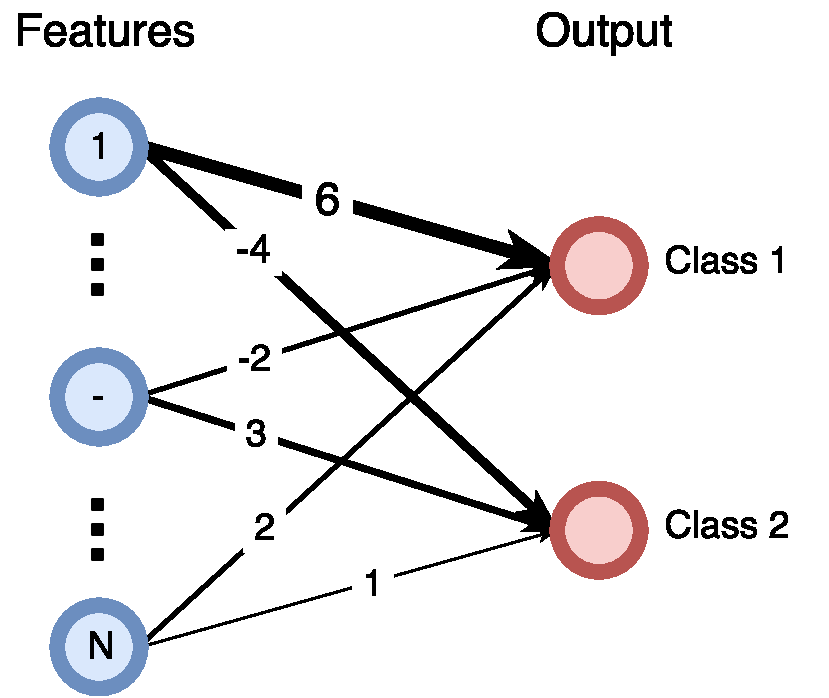
\includegraphics[width=0.5\linewidth]{assets/figures/coefs_example.pdf}%
		\caption[Example: One-layer neural net]{%
			Example of an one-layer neural net. The numbers on the line from input features to the output are weights.
			We examine these weights for single features to gain an insight into the importance the neural net assigned to a given feature. Since a feature contributes to all output neurons, we look at the sum of its absolute weights. Eg. for \textit{Feature 1} the sum of the absolute weights would be $|6| + |-4| = 10$ and for \textit{Feature N} it is $|2| + |1| = 3$, which gives us the hint that \textit{Feature 1} might be more important for the classification result than \textit{Feature N}.
			This analysis presupposes that the feature magnitudes, ie. the values of features, are normalized or - roughly speaking - in the same range on average, eg. \textit{Feature 1} does not take values between $[100, 200]$ while \textit{Feature N} takes values from $[0, 1]$, instead both feature values are roughly in the same range.
		}%
		\label{fig:coefs_example_one_layer}}
\end{figure}

Figure \ref{fig:combined_coefs_l1_l2_regularization} then shows an example of a weight analysis for the \textit{ng20} dataset and for two regularizations, namely \textit{L1} and \textit{L2}.

Both regularization terms are used to discourage ``big" weights, effectively forcing the training algorithm to chose important features to generalize the data instead of over-fitting the data.
While both \textit{L1} and \textit{L2} regularization discourage big weights, \textit{L1} penalizes small weights harder than \textit{L2}, leading to more zero coefficients \cite[p.~13]{Hastie2009}.
Therefore, the selection of important features is enforced more with \textit{L1} regularization.
We leverage this phenomenon to analyze how important the features, graph and text, are for classification.
When looking at the absolute sum of the weights of the trained one-layer neural net, we discover that using \textit{L1} regularization results in the text features becoming more important than graph features for classification.
While the difference of absolute sums of the coefficients does not seem especially high, it has to be noted that graph features are approximately only half as dense as text features.
Thus the contribution by graph features to the end result is even lower than the neural net coefficients indicate.

\begin{figure}[htb!]
	\centering
	{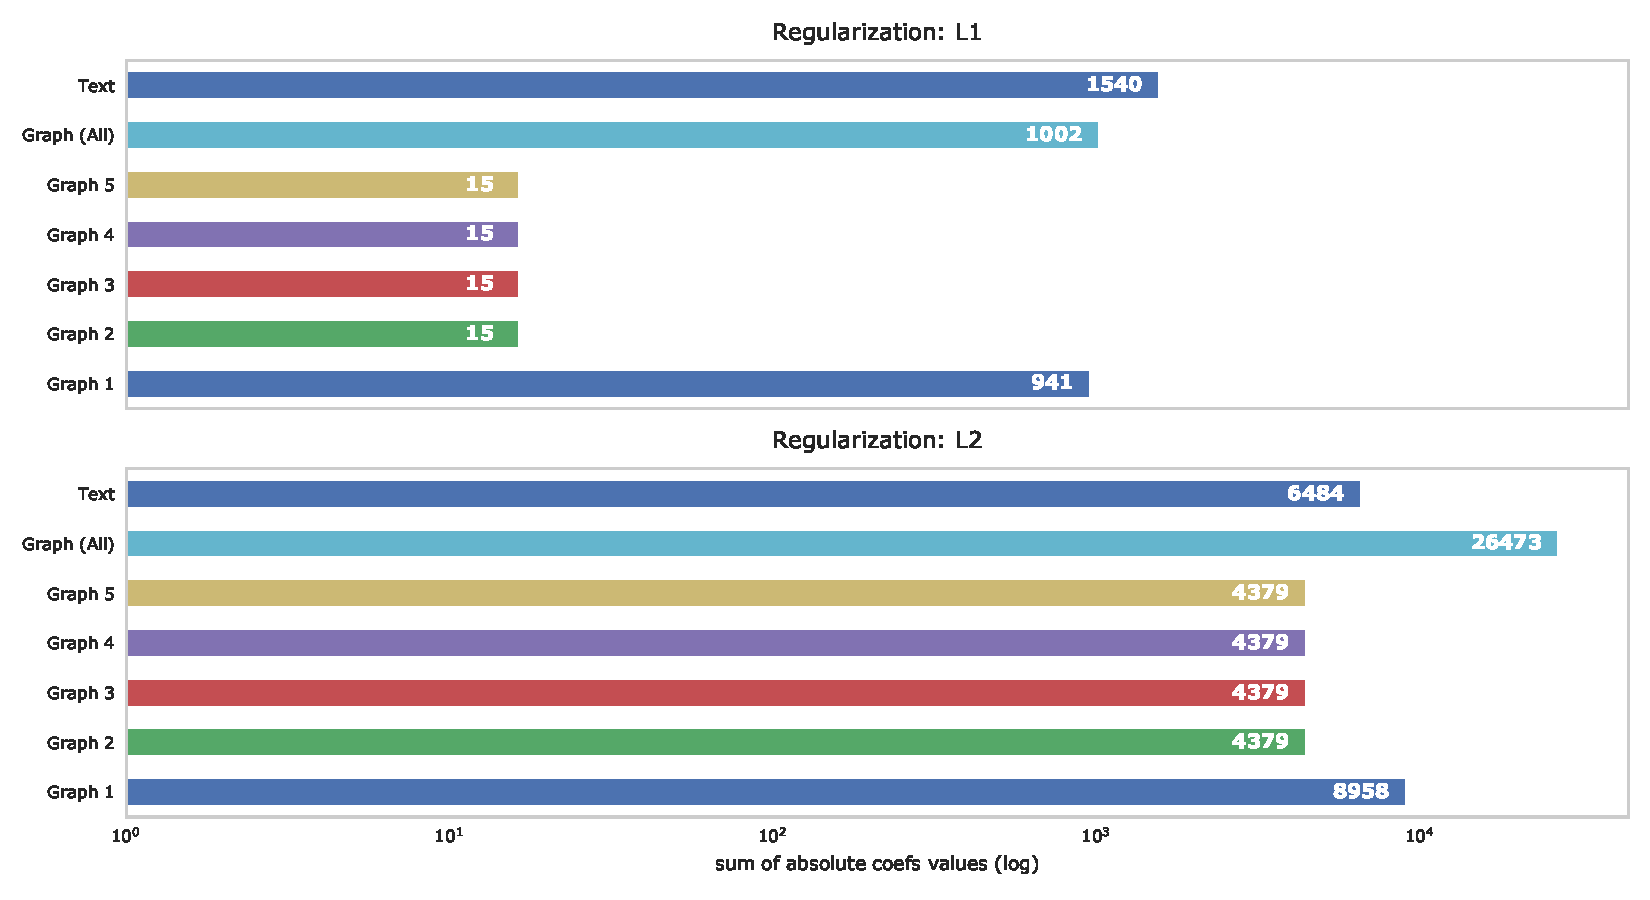
\includegraphics[width=\linewidth]{assets/figures/combined_coefs_l1_l2_regularization.pdf}%
		\caption[Statistics: Histogram of the trained weights of a one-layer neural net]{%
			Histogram of the trained one-layer neural net weights. The neural net was trained on the concatenated graph- and text features.
			Higher values indicate higher importance.
			\textit{Graph (All)} stands for the sum of all graph feature weights, while the \textit{Graph $N$} stand for the individual Weisfeiler-Lehman iterations.
			Higher iterations of WL take a bigger neighborhood into account.
			Dataset: \textit{ng20}.
		}%
		\label{fig:combined_coefs_l1_l2_regularization}}
\end{figure}

Another interesting result of this weight analysis is the importance the neural net assigns to the different Weisfeiler-Lehman iterations. In our example, we chose $h = 5$ for our WL iterations. The higher the iteration, the bigger the neighborhood that is considered by WL.
When looking at the importance of the first iteration and \textit{L1} regularization, \textit{Graph 1} in Figure \ref{fig:combined_coefs_l1_l2_regularization}, we see that while the neural net nearly discourages all higher WL iterations by assigning low weights, it assigns higher importance to the first iteration of WL.
The first iteration of WL takes only the immediate neighborhood into account, therefore matches are far more probable than matches in higher iterations.
In our example in Figure \ref{fig:combined_coefs_l1_l2_regularization}, \textit{L1}- outperformed \textit{L2} regularization by a high margin, approximately 7\% difference in the \textit{F1} macro score.
However, it has to be noted that no hyper-parameter tuning was performed and only a simple train-/test split was used.

\begin{table}[htb!]
\centering
\begin{tabular}{lrrrr|rrrr|r}
	\toprule
	{} & \multicolumn{9}{c}{F1 macro} \\
	{} & \multicolumn{4}{c|}{Concept Map} & \multicolumn{4}{c|}{Co-Occurrence} &  Text \\
	&     Plain & Split & To-Text & Infreq. & Plain & Split & To-Text & Infreq. &  \\
	\midrule
ling-spam       & 0.990 & 0.986 & 0.980 & 0.990 & 0.984 & 0.997 & 0.994 & 0.997 & 0.990 \\
ng20            & 0.791 & 0.737 & 0.756 & 0.781 & 0.672 & 0.694 & 0.712 & 0.694 & 0.781 \\
nyt\_200         & 0.917 & 0.891 & 0.904 & 0.888 & 0.875 & 0.892 & 0.921 & 0.892 & 0.921 \\
r8              & 0.921 & 0.929 & 0.931 & 0.929 & 0.914 & 0.931 & 0.939 & 0.933 & 0.921 \\
review\_polarity & 0.870 & 0.837 & 0.850 & 0.880 & 0.855 & 0.850 & 0.857 & 0.850 & 0.877 \\
rotten\_imdb     & 0.885 & 0.877 & 0.883 & 0.890 & 0.910 & 0.907 & 0.913 & 0.904 & 0.886 \\
ted\_talks       & 0.481 & 0.433 & 0.436 & 0.468 & 0.442 & 0.482 & 0.485 & 0.491 & 0.464 \\
	\bottomrule
\end{tabular}

\caption[Results: Combined text- and graph features]{Classification results for combined graph- and text features classification.
\textit{Split} stands for the WL extension where the multi-word labels are split, see answer to Question \ref{subquestionanswer:question:multi_labels}.
\textit{To-Text} converted the graph back to text, then a classifical Tfidf-BoW approach was used, see answer to Question \ref{subquestionanswer:question:importance_structure}.
\textit{Infreq.} is the WL extension where infrequent nodes are ignored, see answer to Question \ref{subquestionanswer:question:infrequent_nodelabels}.
No significant improvement found over the text-only approach using the permutation test.
}%
\label{table:results_comparison_combined}
\end{table}

\answersummary{
	When combining the graph- and text features we do not achieve no significantly higher classification scores and even observe a degradation.
	Examining the weights of one-layer neural net shows us that, when training on combined text- and graph feature, graph features get lower absolute weights assigned.
	A possible explanation is that the graph features are not as important for the combined text- and graph feature classification.
}

\subquestionref{question:comparison_runtime}
Until now, we only looked at the classification scores of our classification approaches.
Another aspect of great real-world importance is the runtime and memory consumption of these approaches.
In table \ref{table:runtime_and_classifier_size}, we report empirical data on both the runtime\footnote{Machine specification. CPU: \textit{Intel(R) Core(TM) i7-2675QM CPU @ 2.20GHz, Quad-Core, RAM: \textit{8GB}}} and final classifier size of the used pipelines for each dataset.
For this data, we use simple approaches for both graphs and texts: for the \textbf{texts} we vectorize the text documents with BoW with Tfidf.
For \textbf{graphs}, we vectorize the graphs with the plain Weisfeiler-Lehman graph kernel with $h = 4$ iterations.
For both the text- and graph approach, we then train a SVM on the whole dataset, then predict the labels for the whole dataset. Afterwards we save the models, ie. the internal coefficients of the SVM, and record the size of the saved model.
We also record the runtime of both approaches.

As we can see, the graph kernel creates higher dimensional feature vectors for the objects than the text-based BoW approach. 
This observation both give possible explanations for both the higher classifier model size and the run-time.
One could circumvent the higher dimensionality of features extracted by WL by applying dimensionality reduction.
Yet, this would also incur an additional compute overhead and add complexity to the approach.
Preliminary tests with truncated SVD \cite{Mathematics2009} and PCA \cite{Jolliffe2002} to reduce the dimensionality of the graph features resulted in out-of-memory exceptions.

Note, that the reported runtime and memory consumption for the graph-based pipeline does not incorporate the creation of the concept maps, only the creation of the feature maps and subsequent training/prediction.
The creation of concept maps from text with the code provided in \cite{Falke2017b} takes well over a day for our datasets.
For instance, the concept map creation for the documents  in one of the middle-sized datasets, \textit{ling-spam} with 1.2 million words in total and less than 2900 documents, took over 25 hours and had a peak memory usage of 83 Gigabyte\footnote{Machine specification. CPU: \textit{2 $\times$ Intel(R) Xeon(R) CPU X5650 \@ 2.67GHz, 6-Core}, RAM: \textit{190GB}}.
The runtime of the concept map creation could most likely be reduced by parallelizing parts of its pipeline.
For example, the extraction of relevant concepts and their relation from a text is independent from the same extraction of another text, so this stage has neither data- nor functional dependencies.

\begin{table}[htb!]
	\centering
	\begin{tabular}{lrrrrrrrr}
\toprule
		& \multicolumn{2}{c}{Classifier Size} &  \multicolumn{2}{c}{Runtime} &  \multicolumn{2}{c}{Feature Runtime} &  \multicolumn{2}{c}{\# Features} \\
		\midrule
		&  Graph &  Text &  Graph &  Text & Graph &  Text  & Graph &  Text \\
		\midrule
ling-spam       & 11 & 4 & 5 & 2 & 3 & 2 & 246 & 61 \\
ng20            & 143 & 29 & 115 & 10 & 15 & 5 & 750 & 134 \\
nyt\_200         & 90 & 9 & 59 & 8 & 7 & 6 & 1061 & 88 \\
r8              & 28 & 3 & 19 & 2 & 6 & 1 & 282 & 25 \\
review\_polarity & 17 & 3 & 7 & 2 & 3 & 2 & 369 & 40 \\
rotten\_imdb     & 4 & 1 & 5 & 0 & 4 & 0 & 80 & 21 \\
ted\_talks       & 17 & 3 & 2 & 2 & 1 & 2 & 254 & 34 \\
		\bottomrule
	\end{tabular}
\caption[Table: Runtime, classifier size and \# features for graph- and text based classification.]{
	Runtime, classifier size and number of features of text- and graph based classification.
	The feature runtime corresponds to the feature extraction runtime, both for WL for graphs and Tfidf for texts.
	The runtime is reported in \textit{seconds}, classifier size in \textit{Megabytes}, \textit{\# Features} in thousands.
}
\label{table:runtime_and_classifier_size}
\end{table}

\answersummary{
	Graph-based classification using WL incurs both	a runtime and memory consumption overhead to text-based classification.
	One explanation for both the higher memory consumption and runtime is the higher dimensionality of the feature vectors created by WL.
	Applying dimensionality reduction might be a solution to circumvent these issues, yet it has to be noted that the feature vectors are very sparse and are most likely not normalized, so \textit{PCA} is not an option.
	The creation of concept maps from text also incurs a high runtime and memory consumption overhead.
}

\labelsubsection{Summary}{subsec:results_summary}
As we have observed in several of the answers, transforming the text classification task into graph classification and using concept maps is possible.
While we see near state-to-the-art performance with the graph-based approaches, the graph-only performance still lags behind text-only performance as we have seen in the results of Question \ref{question:comparison_text}.
We provided possible explanations in Question \ref{question:structure_diversity}, for example the low connectivity and the high compression factor of concept maps to name just a few.

Questions \ref{question:importance_structure}, \ref{question:multi_labels}, \ref{question:edge_labels}, \ref{question:infrequent_nodelabels}, \ref{question:relabeling_infrequent} and  \ref{question:directed_vs_undirected} all contain approaches to improve the graph-only performance and create more meaningful graph features.
While we, as said before, came close to the classification performance of the text-only approach, there most likely is only so much one can do to improve the classificatio score of concept maps.
In some of these questions, we explored the particularities of concept maps, namely (1) the multi-word node labels, (2) the directed edges and (3) the edge labels.

For (1), we tried splitting the multi-word concepts of the concept maps into single-word nodes.
This resulted in a high increase in classification score.
This was done in \ref{question:multi_labels}.

In Question \ref{question:importance_structure}, we also split the multi-word concepts. We linearized the graph into text again, un-rolling the edges into sentences. Afterwards we used conventional, text-based approaches like BoW to classify the resulting text.
This approach resulted in the best classification performance we achieved using the concept maps, except when combining the graph features with text features.
This observation alludes to the explanation that the structure of concept maps is either not that important for classification or the structure could not be captured usefully using the graph-based approaches we tried.

For (2), the directed edges, we compared the classification results of both directed and un-directed version of the concept maps.
Using the directed edges outperformed the un-directed edges consistently and by a high margin.
We also provided a possible explanation, namely that the neighborhood of a node are far smaller when using directed edges.
Smaller neighborhoods in turn increase the likelihood for matched neighborhoods.

For (3), the edge labels, in Question \ref{question:edge_labels} we first analyzed the distribution of occurrences of edge labels. Here, we observed that most edge labels occur either only once or very often.
The top edge labels, ie. the edge labels which had the most occurrences in the concept maps of a dataset, were almost exclusively non-topic related words, like ``are" or ``is".
Next, we linearized the concept map into text with (a) all words and (b) no edge labels.
Finally, we used a Tfidf-BoW to create features and classify them.
Using or omitting the edge labels resulted in nearly the performance, hinting to the observation that edge labels are not as important for the graph-based approach.

Finally, for the last Question \ref{question:comparison_runtime}, we report the classification times and classifier model size of our graph- and text based approaches.
Here, we observe that the runtime for our graph-based approaches is higher than that for the conventional text-based classification.
We also saw the additional overhead produced by the need to generate the concept maps from the text.

One thing to note, and this is common to all the questions and observations in this work, is that we evaluated our questions on multiple datasets. Often times, the observations differed quite heavily from dataset to dataset.
For instance, the performance of one WL extensions might show great improvement over another on one dataset, while showing a low performance on another dataset. 
Especially when trying to find correlations and explanations for the performance of our approaches, the differing datasets proved to harden the task.
This further highlights the importance of using model selection.
Arguably more than in other domains,  graph-kernel based classification performance relies heavily on the used graphs, structure, graph kernels and particularities of the domain.
We evaluated several other graph kernels, for instance shortest-path- or random-walk based graph kernels, and observed poorer performance than with our default graph kernel, Weisfeiler-Lehman.
Yet, even the Weisfeiler-Lehman kernel with our extensions and several graph pre-processing approaches, we did not outperform the linearized graph approach, ie. where we un-roll the concept map into text then use a conventional BoW-based approach.
A possible explanation for this observation is, that the concept maps are generated from the text by extracting multi-word concepts and their relation to each other from the text.
In order for this approach to create structurally interesting concept maps, concepts have to occur multiple times.
If that is not the case, that is when the concepts occur only once, the resulting concept maps consist of a number of connected components which contain only two nodes and one edge.
These two-node connected components are like tri-grams, with multi-concepts and edge label instead of single-words.

In the next Section \ref{sec:conclusions} we will further summarize our results and provide some approaches we have not tried yet which could further improve the classification scores.

\todo{Mention pros/cons of graph based classification}
\todo{Mention that the questions have not been answered in that order}
\todo{Co-occurrence have little structure, why do they perform better?}

\labelsection{Related And Intermediate Observations}{subsec:related_and_intermediate_observation}
In this section we report observations which are not directly related to our hypothesis, but have provided us valuable insights into our analysis.

\subsection{Weisfeiler-Lehman $\phi$ Feature Map Visualization}
\todo{Add to appendix?}
When debugging our Weisfeiler-Lehman implementation and extensions, we often wanted to see the effect on the resulting feature vectors.
For this, we plotted the feature vector $\phi(G)$ for each graph $G$ for several WL iterations.
In Figure \ref{fig:phi_distribution_example} we see an example of such a $\phi$ distribution plot.

\begin{figure}[htb!]
	\centering
	{\includegraphics{assets/figures/wl_phi_distributions/dataset_graph_concept_map_ng20-v3_phi_npy.png}
		\caption[Example: $\phi$ distribution plot]{%
			Example of a WL $\phi$ distribution plot.
			For each WL iteration $h$, the horizontal $x$-axis corresponds to the concept maps in the datasets, while the vertical $y$-axis corresponds to the indices of $\phi(G)$ which are non-zero, ie. when there is a point at $x=0$ and $y=10$, the graph $G_0$ has the label $10$.
			There are as many points in this plot as there are vertices in the dataset.
			The colors of a point corresponds to the class of the graph, in this case the 20 classes of \textit{ng20}.
			The red line marks the number of vertices in the datasets which is also the dimension of the feature map $\phi$.
			Dataset: \textit{ng20}.
			\textit{Note: embedding this plot in a vector format  was not possible due to the sheer number of points to be drawn. The rasterized image seen here interpolates the individual points.}
		}%
		\label{fig:phi_distribution_example}}
\end{figure}

It has to be noted that we implemented WL where the labels are assigned when they are first encountered. That means that when we create the feature map $\phi(G_i)$ for graph $G_i$, we relabel the graph by assigning it a new multi-label by taking the neighborhood into account (\textit{recoloring}). In the next step, we compress the new multi-label by assigning it a new number if it has not been encountered before and save it in a multi-label-lookup. If the multi-label has been encountered before, ie. the multi-label is in the multi-label-lookup, we assign it the number it has been assigned before.
This is the \textit{label compression} step.
So, we iterate over the graphs one by one and create feature maps $\phi$.
When the first processed graph, $G_1$, has the new compressed labels $\{1, 2, \ldots, n\}$, the next processed graph, $G_2$, will have labels that are either \textbf{(1)} new, in which case they get a new, compressed label that is higher than $n$ or \textbf{(2)} they were already encountered in $G_1$, so they get the label from the lookup.
This way we get incrementing labels for each graph.
When we also sort the graphs by their assigned class, ie. all graphs of class $y_i$ are processed after another, then one can look at the labels that are assigned to each class and also see the nice pattern which arises in Figure \ref{fig:phi_distribution_example}.

This plot also gives an insight about the convergence of WL.
The highest encountered $\phi$ index in iteration $h=1$ must be higher or equal than the highest $\phi$ index encountered in $h=0$.
This is directly due to the fact that more colors are needed to color the graph nodes in higher iterations - if WL has not converged.
The number of labels, or colors, $|L_i|$ assigned in iteration $h=i$ must be smaller or equal than the labels for iteration $h=i+1$, ie. $|L_i| \leq |L_{i + 1}|$.
When $|L_i| = |L_{i + 1}|$, WL is said to have converged, ie. the number of colors will not change anymore.

In this figure, there is also a highest horizontal, green line.
This line signifies the highest $\phi$ index where there was a non-zero entry.
It also serves as a marker of the last compressed label number which was assigned in this dataset.

While this kind of plot is useful for analyzing the whole datasets at once, it becomes especially interesting when splitting the dataset into sets, eg. by splitting it into a stratified train- and test set.
When creating the feature maps $\phi$ for the graphs in the train set, for each WL iteration $h$ we save the multi-label-lookup which we is then used to create the feature maps for the test set.
The multi-label lookup therefor acts as a kind of continuation, saving the state of the WL iteration with all encountered labels.
Then, when creating the feature maps for the test set, we use the multi-label lookups to generate the feature maps in the same way, now for the graphs in the test set.
When plotting the train- and test set feature maps separated we can get interesting insights into the dataset and the concept maps.
For an example, see Figure \ref{fig:phi_distribution_train_test}.

\begin{figure}[htb!]
	\begin{subfigure}[t]{.49\linewidth}%
		{\includegraphics{assets/figures/wl_phi_distributions/dataset_graph_concept_map_ng20-v3_splitted_phi_npy_train.png}}\caption{Train}%
	\end{subfigure}%
	\begin{subfigure}[t]{.49\linewidth}%
		{\includegraphics{assets/figures/wl_phi_distributions/dataset_graph_concept_map_ng20-v3_splitted_phi_npy_test.png}}\caption{Test}%
	\end{subfigure}%
	\caption[Diagram: $\phi$ distribution plot for \textit{ng20}.]{WL $\phi$ distribution with a stratified train/test split.}%
	\label{fig:phi_distribution_train_test}
\end{figure}

While the train set looks nearly the same as if plotting the simple dataset without the split, the test set differs quite a bit.
Notice how, in the test set, there are ``clusters" around some regions for each of the classes. 
Keep in mind that the $y$-position of the point signifies a non-zero entry at index $i$ in $\phi(G)$ for that graph.
Because of the aforementioned implementation, we now are able to see a pattern for each of the classes, namely the clusters.
For the test set, we can also see how many new labels have been found in a given iteration.
As we said before, the horizontal green line, in both plots, signifies the last label that has been encountered.
In the case of the split sets, it also marks the last label that has been encountered in the train set.
All points, that is labels, above this line have are new to the test set and do not occur in the train set.

Plotting the $\phi$ distribution like so, we gain a better insight into the graph connectedness and the similarity or uniqueness of neighborhoods.
When WL converges at iteration $h$, so when the height of the green line does not change from iteration $h-1$ to $h$, this means that all neighborhoods that are different, have been marked as so and got a unique label.
If the number of labels is equal to the number of vertices, all neighborhoods are different.

\subsection{Weisfeiler-Lehman Node Weighting Extension}
With increasing iterations $h$ of the Weisfeiler-Lehman algorithm, exact matches of subtrees of height $h$ become more difficult.
In iteration 0, WL only counts the number of node labels in the graphs, for iteration 1 it takes the immediate neighborhood of the nodes into account, for iteration 2 is takes the neighborhood of the neighborhood into account and so on.
As a result, \textbf{(1)} with higher iterations, the probability of having an exact match decreases. Another difficulty arises for nodes with a high number of neighbors. \textbf{(2)} The probability of an exact match also decreases with a higher degree.

These two difficulties, \textbf{(1)} the increased difficulty of a match with higher iterations and \textbf{(2)} the increased difficulty of a match for nodes with higher degrees, are not addressed when using Weisfeiler-Lehman in its plain version. Both issues are encoded neither in the features maps nor are they considered when creating the gram matrix.

As a possible solution for these issues, we propose an extension to the Weisfeiler-Lehman algorithm.
Our extension augments the WL algorithm by adding node weights.
For each of the nodes in all graphs, we first calculate node weights which encode the importance of the nodes or the difficulty of getting an exact match in WL.
An example of such node weights are the node degrees or node weights extracted by the \textit{PageRank} algorithm \cite{Page1998}.
The node degree is an interesting metric for node weights since it actually encodes the size of the immediate neighborhood of a node and therefore could possibly address both difficulty \textbf{(1)} and \textbf{(2)}.

One could see our extension as similar to binary \textit{BoW}, ie. only using whether a word has occurred or not, and the extension that also uses the term frequency where the number of occurrences is taken into account, too.

When using this extension, one has to be careful with feature scaling. As we use the node weights to scale individual features, using a separate feature-wise scaler would effectively revert our weighting.

\todo{Explain how to actually use the node weights.}

\paragraph{Experiment}
To test our extension, we compare results of the WL algorithm with and without our extension.
We classify our concept maps datasets as well as a number of other graph benchmark datasets, obtained from \cite{Kersting2016}.
For statistics about the additional datasets, please consult the authors website\footnote{\url{https://ls11-www.cs.tu-dortmund.de/staff/morris/graphkerneldatasets}}.
We used only datasets from the website consisting of more than 1000 graphs and node labels.

\begin{table}[htb!]
	\centering
\begin{tabular}{lrrr}
\toprule
	{} & \multicolumn{2}{c}{F1 macro} & {p-value} \\
	{} &  plain &  node weights &  \\
	\midrule
	ling-spam       & \textbf{0.8160} & 0.7760 & 0.0542 \\
	ng20            & \textbf{0.4188} & 0.4127 & 0.2340 \\
	nyt\_200         &\textbf{ 0.7436} & 0.7150 & 0.3421 \\
	r8              & \textbf{0.6772} & 0.6467 & 0.1270 \\
	review\_polarity & \textbf{0.6094} & 0.6045 & 0.8406 \\
	rotten\_imdb     & \textbf{0.6346} & 0.6338 & 0.8728 \\
	ted\_talks       & 0.2436 & \textbf{0.2984} & 0.2605 \\
	\midrule
	AIDS             & 0.9560 & \textbf{*0.9841} & 0.0146 \\
	DD               & 0.6602 & \textbf{*0.7733} & 0.0002 \\
	Mutagenicity     & \textbf{0.7702} & 0.7625 & 0.3007 \\
	NCI1             & \textbf{0.8425} & 0.8334 & 0.2821 \\
	NCI109           & \textbf{0.7929} & 0.7877 & 0.4971 \\
	PROTEINS         & 0.7266 & \textbf{0.7317} & 0.8554 \\
	%PROTEINS\_full    & 0.7266 & \textbf{0.7317} & 0.8574 \\
	Tox21\_AHR        & 0.7009 & \textbf{0.7056} & 0.6705 \\
	Tox21\_AR         & \textbf{0.8147} & 0.7978 & 0.1172 \\
	Tox21\_AR-LBD     & \textbf{*0.8477} & 0.8284 & 0.2318 \\
	Tox21\_ARE        & 0.6722 & \textbf{0.6917} & 0.1378 \\
	Tox21\_ATAD5      & \textbf{0.7456} & 0.7426 & 0.7449 \\
	Tox21\_ER         & \textbf{0.6860} & 0.6747 & 0.0868 \\
	Tox21\_ER\_LBD     & \textbf{0.7335} & 0.7180 & 0.0648 \\
	Tox21\_HSE        & 0.6156 & \textbf{*0.6499} & 0.0384 \\
	Tox21\_MMP        & 0.7663 & \textbf{0.7682} & 0.7874 \\
	Tox21\_PPAR-gamma & \textbf{0.7006} & 0.6910 & 0.7970 \\
	Tox21\_aromatase  & 0.6571 & \textbf{0.6876} & 0.1642 \\
	Tox21\_p53        & 0.7214 & \textbf{0.7375} & 0.3403 \\
	\bottomrule
\end{tabular}
\caption[Results: Classification using node weight WL extension]{F1 macro classification results for  the node weight extension.}\label{table:wl_node_weight_extension}
\end{table}

As we can see, the classification performance of our extension varies greatly per dataset.
Especially on the concept maps, our WL extension does not perform as good the plain WL graph kernel.
On some of the graph benchmark datasets, we can also observe significant improvements.
 
\if
We also tried another extension to the Weisfeiler-Lehman graph kernel, namely augmenting the default node label counts with a iteration factor.
The feature maps of WL consist of the concatenated feature maps for each iteration.
For this extension, we propose weighting the feature maps of each iteration $h$ by a factor given by a function $f(h)$.
So, for a feature map, $\phi(G)$, of a graph $G$ for $h=2$ iterations, the feature map can be decomposed into the feature maps of each of the two $h$ iterations:
\begin{equation*}
\phi(G)=(\phi_{h=1}(G), \phi_{h=2}(G))
\end{equation*}
We now propose to weight the individual feature maps by the factor determined by function $f(h)$, so:
\begin{equation*}
\phi_{f}(G)=(f(1) \cdot \phi_{h=1}(G), f(2) \cdot \phi_{h=2}(G))
\end{equation*}
So, basically the function $f(h)$ works as a decaying factor to decreasing iterations $h$.
When the function $f(h)$ increasing, the increasing importance with higher iterations is encoded into the resulting feature map $\phi_f(G)$.
Of course, also this extension 
\fi